\documentclass{beamer}

\usepackage[utf8]{inputenc}
\usepackage{subfiles}
\usepackage{animate}
\usepackage{pgfplots}
\usepackage{subcaption}
\usepackage[german]{babel}
\usepackage{siunitx}
\usepackage{chemfig}
\usepackage{listings}
\usepackage{graphicx}

% Tikz
\pgfplotsset{compat=1.17}
\usetikzlibrary{decorations.pathmorphing}
\tikzset{wavy/.style={decorate, decoration=snake}}

\title{Entwicklung eines Infrarotspektrometers}
\author{Noah Jutz}
\institute{Privat-Gymnasium PINDL Regensburg}
\date{2020-12-07}


\begin{document}

\frame{\titlepage}

\begin{frame}
    \frametitle{Gliederung}
    \tableofcontents
\end{frame}

\section{Motivation}
\subfile{sections/motivation.tex}

\section{Grundlagen}
\subfile{sections/grundlagen.tex}

\section{IR-Spektrometer}
\subfile{sections/ir_spektrometer.tex}

\section{Erfahrung}
\subfile{sections/erfahrung.tex}

\setbeamertemplate{background canvas}{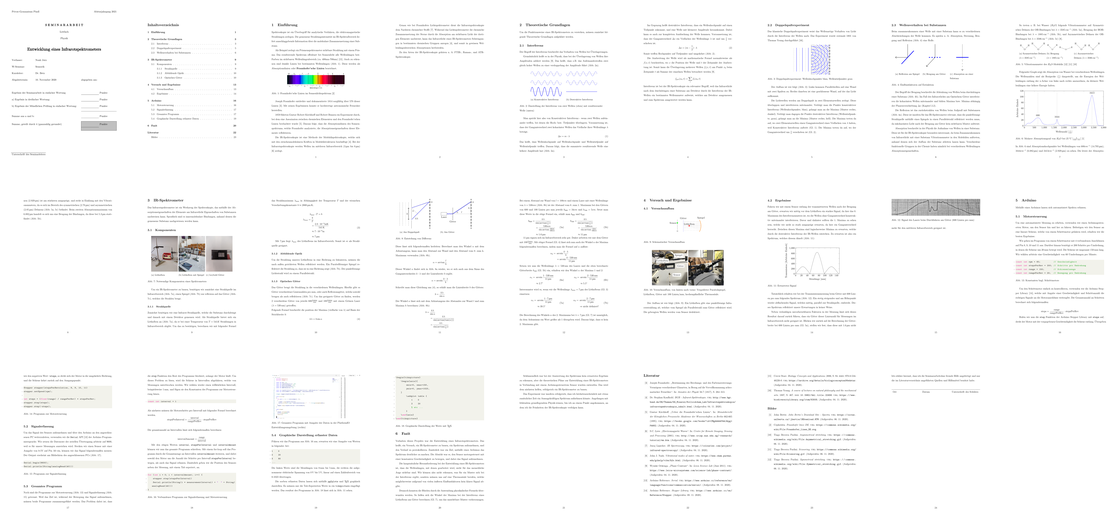
\includegraphics[width=\paperwidth,height=\paperheight,keepaspectratio]{assets/images/seminararbeit_collage.png}}
\frame{}

\end{document}
